\section{Interview with customer representatives 13/3}\label{interview13-3}
During pre-sprint 1 and the beginning of sprint 1, a lot of changes and design updates were considered for the interface of GIRAF.
This resulted in new prototypes, icons and a revision of the previous design guide used for the project.
To evaluate the changes made, we invited customer representatives to come for an interview and a presentation of the changes.
This interview was scheduled to take place on March 13th.
Two representatives from different partners were able to make this meeting - Susanne from Birken and Mette from Egebakken.

\subsection{The interview structure}
The primary goal of the interview was to confirm that the changes made to the design were acceptable.
The secondary goal was to clarify certain uncertainties we encountered.
The prototypes that had changed and needed feedback were related to the following functionalities of GIRAF:
\begin{itemize}
    \item The timer functionality
    \item Pictogram search
    \item Different ways of marking activities as done
    \item Copying a week plan to a different citizen
    \item The redesign of the login screen with citizen selection
    \item Greyscale functionality
    \item Showing different amounts of days
    \item Horizontal view of week plan
    \item Marking multiple activities at the same time
\end{itemize}

\subsection{The key points of the interview}
The discussions that arose based on the presentation led to valuable information.
The most essential will be discussed below.

\subsubsection{Copying week plans between citizens and the login screen with citizen selection}
These two prototypes illustrated the fundamental functionality of the weekplanner.
The representatives were happy with the design as shown on the prototypes, however they had some concerns with the selection of citizens.
Susanne and Mette were worried that there might be too many layers to this functionality.
If they would have to go through multiple layers to insert pictures to get it to display as shown on the prototype, they would not be thrilled.
They wanted it to be accessible and very intuitive.
\\\\
Another concern brought up is the need to be able to divide the citizens in a way that makes sense for the guardians.
Generally, the guardians are only concerned with a select number of citizens.
Proposed solutions to this as discussed with the representatives was to either add a search functionality for selecting citizens, or add a new layer to the prototype and application that worked like a folder system, each folder specifying a class.
\\\\
In regards to copying activities, we discussed whether every citizen had a unique week plan or if one week plan could be assigned to multiple citizens.
Susanne and Mette remarked that usually a foundation can be used.
Mette also specified that Egebakkens schedule is based on a template that changes depending on the week.
On even weeks they would go horseback riding, while on odd weeks they would do another activity.

\begin{figure}[!htb]
    \center
    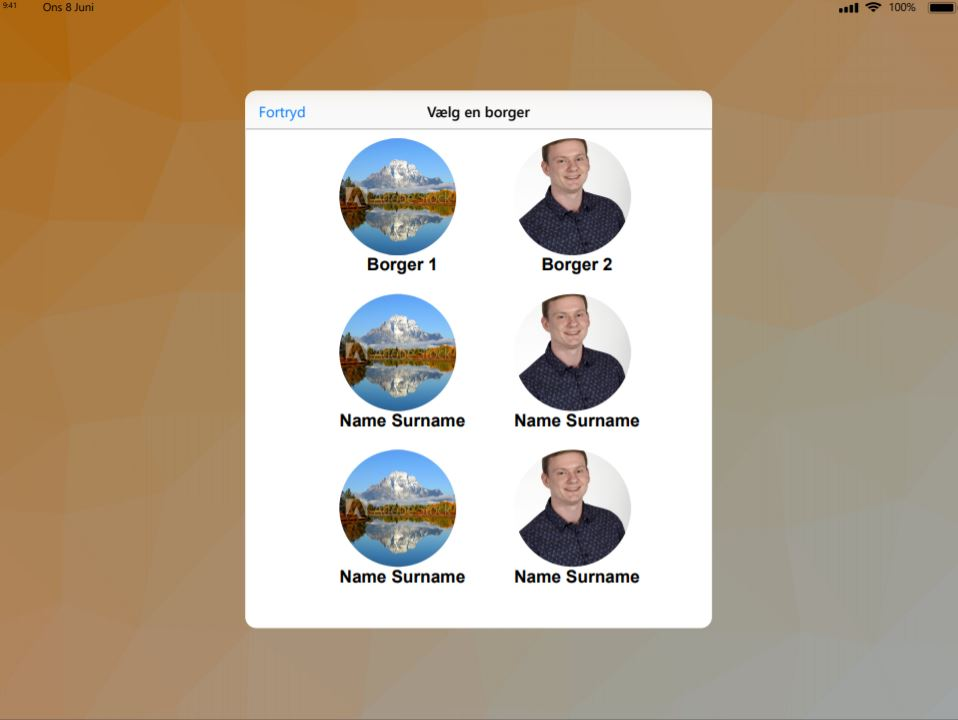
\includegraphics[width=0.8\textwidth]{figures/select-citizen.JPG}
    \caption{\label{fig:choose-citizen-prototype} Prototype of choosing a citizen.}
\end{figure}

\subsubsection{Showing different amounts of days}
The functionality of showing different amounts of days posed some uncertainties.
GIRAF should be able to show seven days, five days, three days or just one day at a time, based on requirements defined by last year's development team.
However, if the application were to show five days ahead, and the current day were Friday, how would it handle the overlap with the next week?
This question was discussed for a while, eventually leading to the conclusion that if this were the case, they would want the application to show the next days, even if they might overlap with next week.
The problem that these days might be empty, as a plan might not have been made for the coming week, is ultimately a problem they would have to deal with on their end.

\subsubsection{Marking activities as completed, manipulating multiple activities and searching for pictograms}
In terms of marking activities as completed, they were happy with the options we presented.
The ability to manipulate multiple activities at a time would be nice to have.
The prototypes we had prepared for this functionality were acceptable, however this functionality gave rise to an important discussion.
The institutions want the citizens to be as independent as possible - this means they are the ones that mark activities as completed.
Based on our impressions of the work of previous years on the GIRAF project and the prototypes that were handed down to us, we had thought the guardians would be performing this task.

\subsubsection{The timer functionality}
The requirements of the timer functionality were discussed alongside the prototypes.
Generally, they will add the timer as they add the activities to the week plan, rather than when the activity starts.
\\\\
The different representations of time we had designed were proposed and evaluated.
Generally they wanted to use an hourglass or a circle.
When adding a timer, they would rather input the time the activity takes in minutes than the time period in which the activity takes place.

\begin{figure}[h!]
  \center
  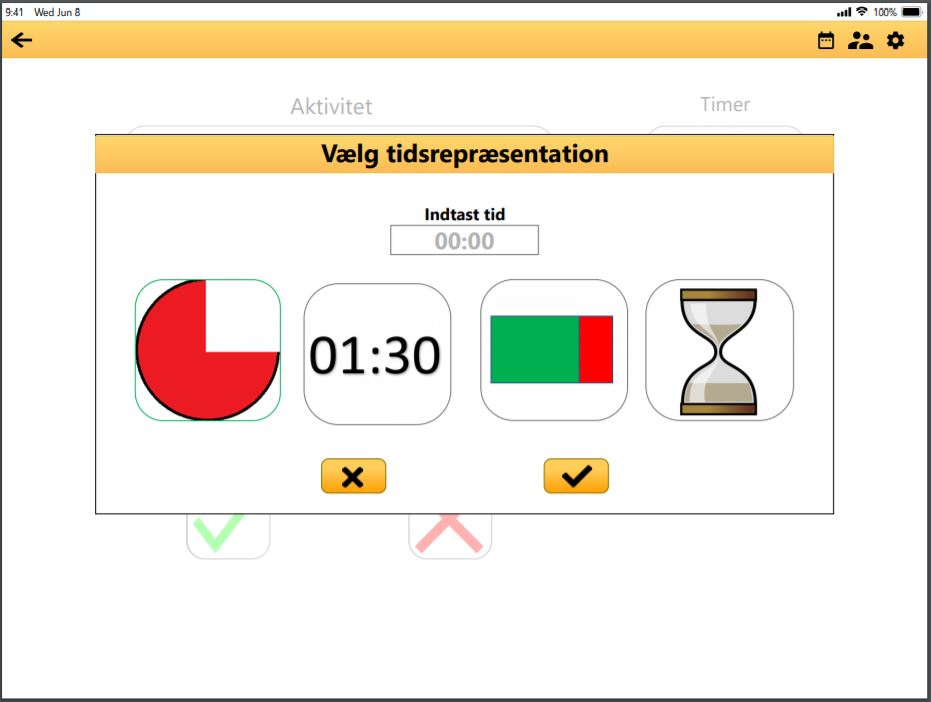
\includegraphics[width=0.8\textwidth]{figures/select-timer-prototype.JPG}
  \caption{\label{fig:choose-timer-prototype} Prototype for choosing a timer.}
\end{figure}

\subsection{Summary of the interview}
The most essential piece of information gained was the fact they we had misunderstood the way activities are marked as completed.
We thought the guardians would perform this action, but it is actually the citizens.
This meant the prototypes needed changing.
When selecting a citizen, an additional layer to divide them into classes would be preferable according to the representatives.
Generally, the designs proposed on the prototypes were acceptable, and the icons used were satisfactory.
